\documentclass[conference]{IEEEtran}
\IEEEoverridecommandlockouts
% The preceding line is only needed to identify funding in the first footnote. If that is unneeded, please comment it out.
%Template version as of 6/27/2024

\usepackage{cite}
\usepackage{amsmath,amssymb,amsfonts}
\usepackage{algorithmic}
\usepackage{graphicx}
\usepackage{textcomp}
\usepackage{xcolor}
\usepackage{svg}
\def\BibTeX{{\rm B\kern-.05em{\sc i\kern-.025em b}\kern-.08em
    T\kern-.1667em\lower.7ex\hbox{E}\kern-.125emX}}
\begin{document}

\title{A Monolithic Electronic-Photonic Platform in Conventional Silicon Photonics Processes\\
\thanks{The authors want to acknowledge the financial support of the NSREC and Alireza Geravand, Sammy Noel-Parisé and Francesco Zanetto for useful discussions.}
}
\author{\IEEEauthorblockN{Philippe Arsenault and Wei Shi$^*$}
\IEEEauthorblockA{\textit{Department of Electrical and Computer Engineering, COPL, Université Laval, Québec, Canada} \\
$^*$wei.shi@gel.ulaval.ca}
}

% Define the macro
\newcommand{\CitationNeeded}{\textcolor{red}{\setlength{\fboxsep}{1pt}\colorbox{yellow}{[citation needed]}}}
% Define the macro
\newcommand{\Value}{\textcolor{red}{\setlength{\fboxsep}{1pt}\colorbox{yellow}{[Missing Value]}}}
\newcommand{\MFig}{\textcolor{blue}{\setlength{\fboxsep}{1pt}\colorbox{green}{[Missing Figure]}}}

\maketitle

\begin{abstract}
We present the design methodology to make any active silicon photonics node, a monolithic platform. 
The approach is based on the usage of the waveguide and complementary dopant to create MOSFETs and digital gates allowing the inclusion of basic on-chip processing and specialized analog circuitry.

\end{abstract}

\begin{IEEEkeywords}
Silicon photonics, Monolithic integrated circuit, electronic-photonic co-design, CMOS integrated circuits
\end{IEEEkeywords}

\section{Introduction}
State-of-the art monolithic electronic-silicon photonics processes are a monumental advancement in the co-design of electronic and photonics circuits.
For high speed application, sharing the same substrate has its advantages: no interconnection needed reducing the parasitic load, integrated simulation environment and simpler mechanical assembly of the integrated circuit (IC) into more complex systems.
Although, at the moment, even the best monolithic processes struggle to compete with recent CMOS nodes in terms of maximum frequency of operation for digital signal processing or the driving power needed for optical modulators. 
For lower speed application that do not need these higher speeds or driving power, monolithic nodes seems to be an enticing solution for its ease of use, embedded testing capabilities and easier physical assembly.
Nevertheless, since monolithic nodes are usually build upon an existing CMOS node and modified to fit the less strainuous fabrication of the photonics, they tend to exceed the price per area of similar CMOS processes\cite{shekhar_roadmapping_2024}. 

Integrating CMOS capabilities in a silicon photonics node, although possible, is relatively new. 
It creates a new avenue to access a monolithic node for researchers and industry without the high entry price.
Prior art has shown that integrating CMOS transistors into a conventionnal silicon photonics process is possible but limited\cite{zanetto_unconventional_2023,shekhar_roadmapping_2024}, as it shows poorer electrical performances than equivalent CMOS and has no foundry supplied electronic libraries.
It has more recently been used in power monitoring and signal multiplexing applications\cite{crico_monolithic_2024,zanetto_timemultiplexed_2023}.

In this paper, we aim to expand on the idea by proposing improvements on the transistor design, discussing the limitations and pitfalls of the implementation and tooling, and present the progress made towards a monolithic electronic platform in a conventional silicon photonics process.



%It forces the designers of integrated circuit systems to either choose multiple technologies, one dedicated for photonics and others for the CMOS DSP and slow control, and have the challenge of doing the co-design and interconnect or bend to monolithic . 
%As such, a system designer would want to use their monolithic area as best as they can, but they are confronted by three 
%The larger size of the silicon photonics circuits compared to their CMOS counterpart means that one pays the monolithic premium price 


%As the process is geared toward both CMOS and optical capabilities, the price of the area is superior to thoses of either the similar size CMOS or similar performance silicon photonics. 
%This creates a difficult choice for designers who wishes to make an integrated circuit system, either choose two technologies, one for the photonics and the other for the CMOS, and have the hassle of doing the co-design and interconnect or choosing the monolithic process and pay the increased price.


\begin{figure*}[t]
    \centering
    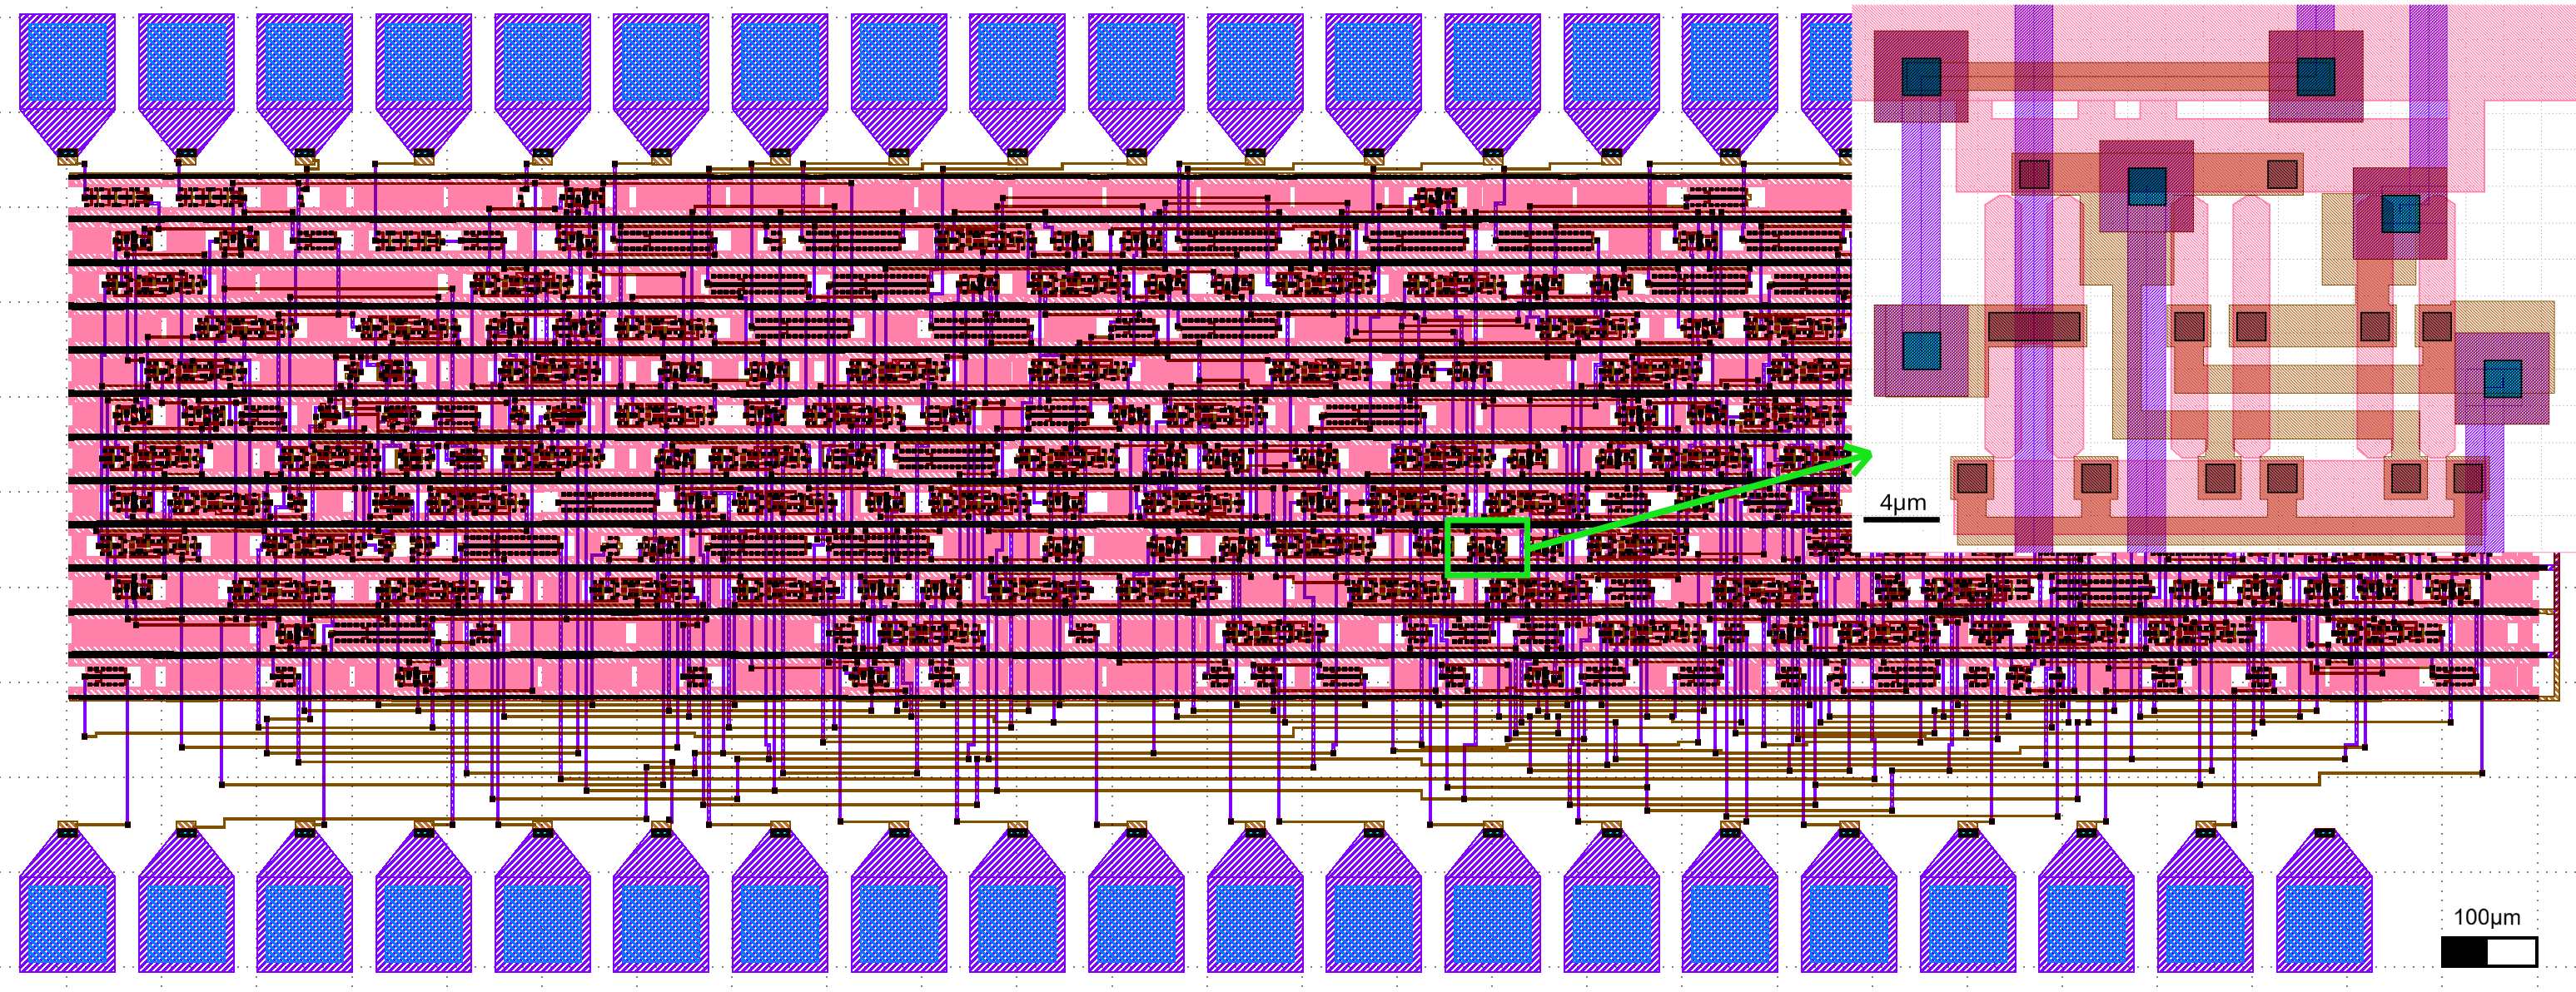
\includegraphics[width=\textwidth]{Core.png}
    \caption{A. The proposed digital core schematic, 
    B. The digital core in a photonics system,
    C. Layout of the digital Core, the inlet shows the detail of a singular digital gate,
    D. A zoomed view of a single NMOS transistor and
    E. The 3D-view of a NMOS transistor beside a waveguide. The waveguide has a germanium photodetector on top.   
    }
    \label{fig:Core}
    \vspace{-10pt}
\end{figure*}

\section{Implementation}
The proposed approch in this article is to give the photonics chip the ability to communicate digitally with an external controller, fixing the number of external connections. 
The Fig.\ref{fig:Core}.A shows the proposed architecture of an electronic-photonic integrated circuit with an internal core driving photonic structures with a DAC and an array of sample and hold circuits, and receiving signal from power monitor photodetectors with an ADC, a transimpedance amplifier and an analog multiplexer. 
The analog circuits can be made directly with the transistors while the mixed and digital circuits need more tooling to be possible. 
Thus, a digital electronic kit was created.
It was then fed into an open-source automated router, OpenROAD\cite{ajayi_openroad_2019}, along with the verilog design files and the technology files. 
The conceptual schematic of the core is shown in Fig.\ref{fig:Core}.B while the layout is shown in Fig.\ref{fig:Core}.C.

Some challenges did arise, one file we were not able to provide to the router yet is the timing library of the gates, which can either be simulated by parasitic extraction simulations or constructed via a measurment campaign.  
Nevertheless, not having the exact timing of the gate influences the maximum clock frequency of the circuit, not its logics, as the circuit will still be capable to compute at a lower speed than expected. 
Additionnaly, during our first measurment campaign of the reduced $L$ and smaller gap transistors, a flaw in the fabrication process was discovered. 
Since the photonics nodes care much more about the optical properties of the waveguides, when we closed the gap between the channel and the gate,a significant amount of the transistor exhibited an unwanted electrical connection was made between the gate and the drain/source or channel, meaning that the device was unusable with the minimal distance prescribed by the foundry. 
Finally, while the size of the Fig.\ref{fig:Core}.C is large, shrinking it is not limited by the physics of the implementation but rather the foundry's tolerances on vias and metals.
 





\section{Fundamentals and Principle}
\begin{figure*}[t]
    \centering
    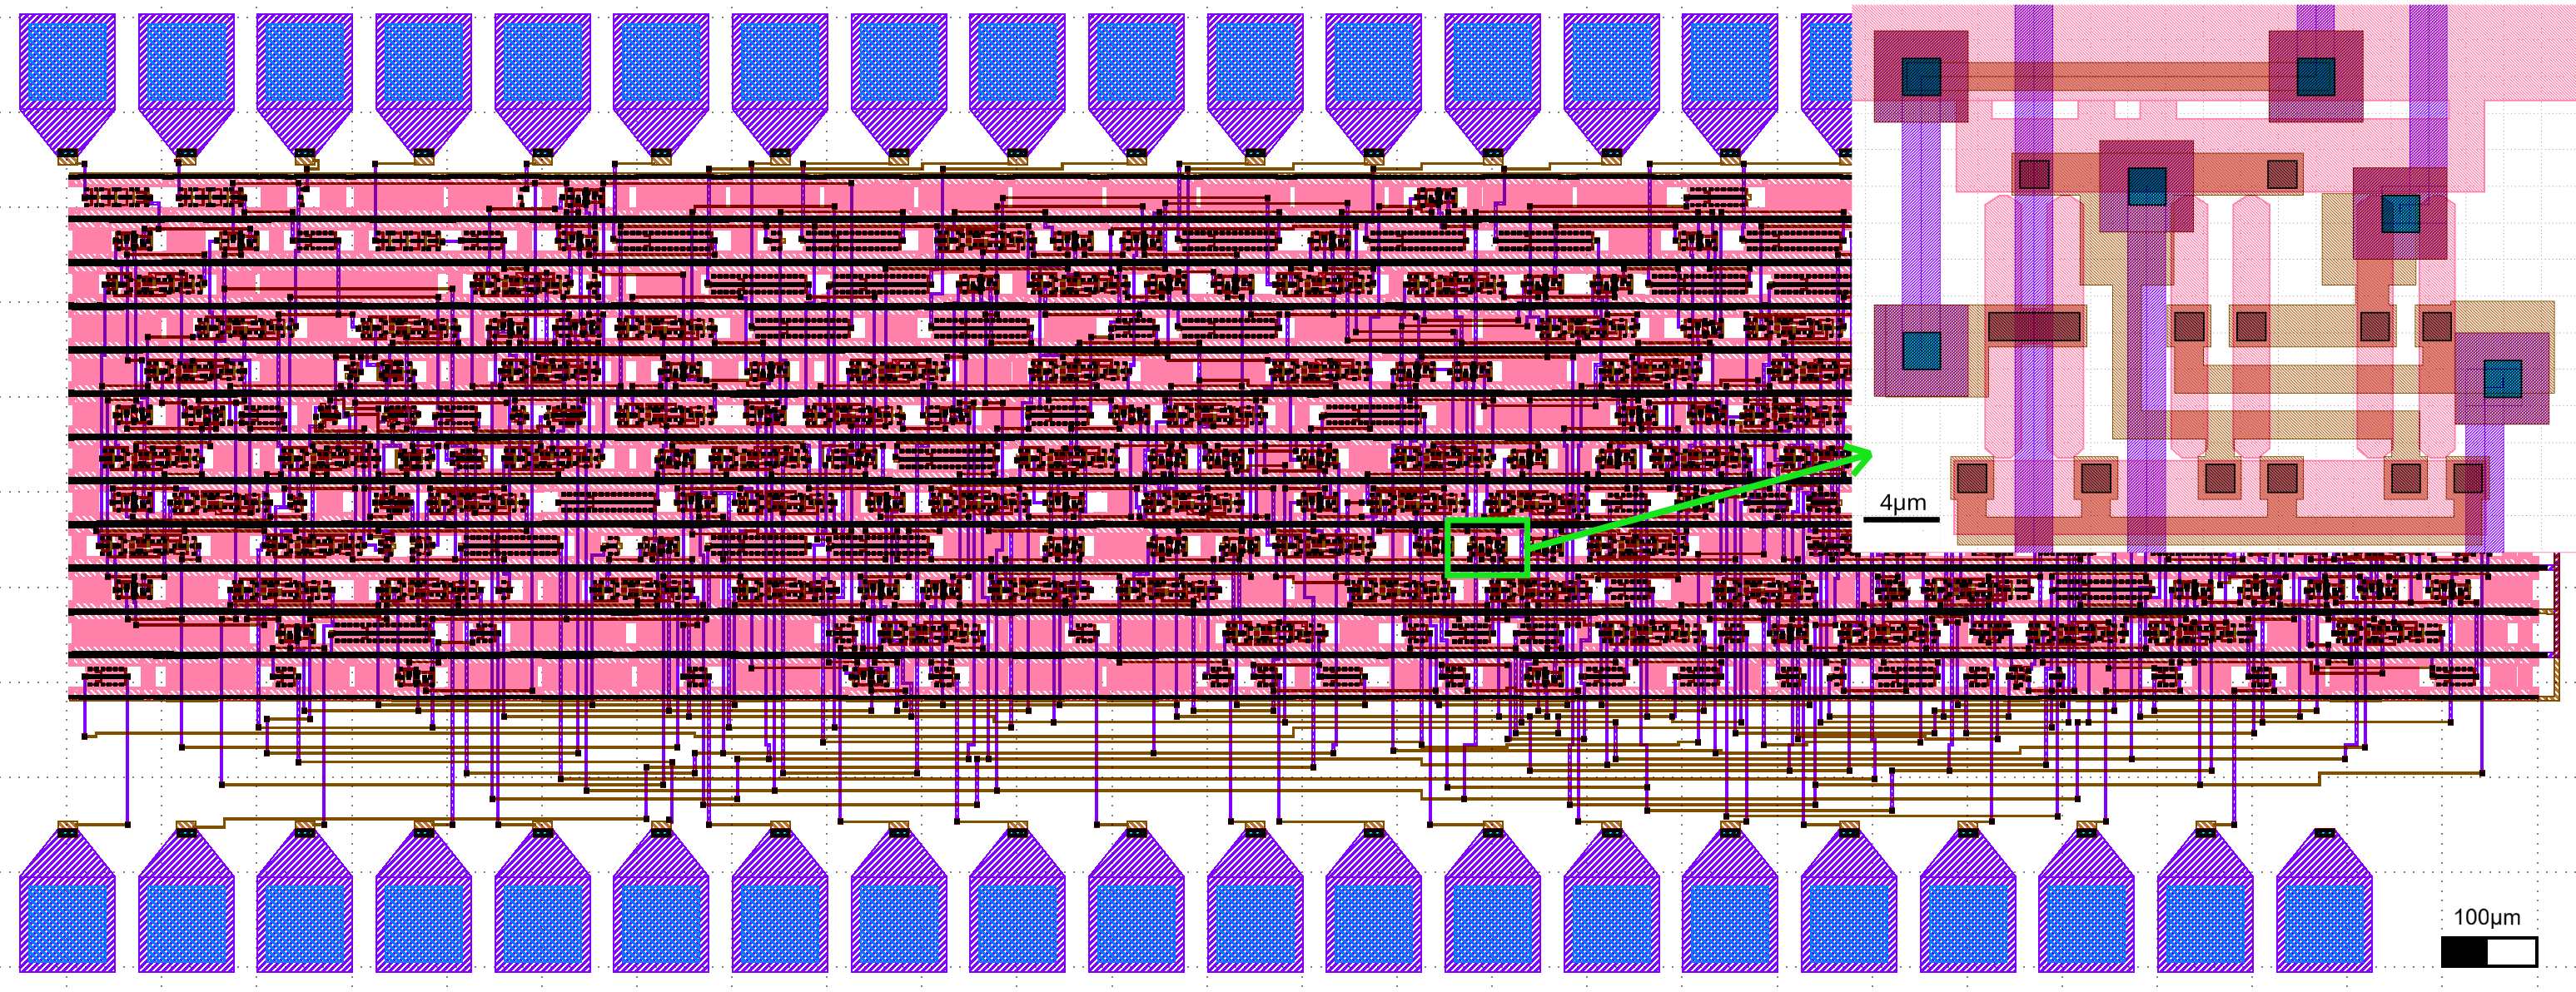
\includegraphics[width=\textwidth]{Core.png}
    \label{fig:Core}
    \caption{A. The proposed digital core schematic, B. The digital core in a photonics system and C. Layout of the digital Core.}
\end{figure*}

While the design of the basic transistor unit is a promising start, improving the design is favorable to the integration of on-chip more complex analog and digital electronics.
This section will present the modeling of the transistors and the effect of the proposed changes has on key parameters; the small signal gain ($gm$) and the cut-off frequency ($F_t$) and their effect on both analog an digital circuits.

A higher small signal gain means that the analog circuitery requires less transistors for the same amplification factor, shrinking the circuits and parasitics. 
The increase of the small signal gain also increases the current output strength of digital gates, helping in the charge and discharge of capacitive loads, such as gates or PN junctions. 
The other parameter, the cut-off frequency of the transistor, is a measurment of how fast a single transistor can switch.
Improving the cut-off frequency of the transistor opens up the design area for analog and digital circuitry as it represents the upper limit at which a circuit can run in a parasitic-less environment.  

The saturation region small signal gain is the measurment of how much the drain current ($I_D$) changes in relation with the gate-to-source voltage ($V_{GS}$) in a specific condition of the drain-to-source voltage ($v_{DS}$).

\begin{equation}
\label{eq:gm}
gm = \left.\frac{\delta I_D}{\delta V_{GS}}\right|_{v_{DS}} = \mu_x C_{ox}\frac{W}{L}(V_{GS}-V_T)(1+\lambda v_{DS})
\end{equation}

In \ref{eq:gm}, $\mu_x$ is the mobility of the charges, $C_{ox}$ is the oxide capacitance per unit area, $W$ and $L$ are the size of the gate, $V_T$ is the threshold voltage and $\lambda$ is the channel-length modulation parameter. 
%In  conventionnal silicon photonics process, the $W$ value is the height of the waveguide, hence the designer only has access on controlling the bias point via  $V_{GS}$ via an external application, and the length $L$ and the oxide capacitance $C_{ox}$ up to their respective manufacturing limit.
The length of the transistor is controllable by the distance between two tubs of the same type of doping and the length of the gate while the width is fixed by the waveguide layer height.
As the physical limit of the gate length is the minimal width of a silicon waveguide, the limiting factor is often the minimal distance between two tubs of similar doping without causing a unwanted connection between the source and the drain.
Depending on the foundry used, this distance can vary and be subject to mask alignment precision. 
As for the $C_{ox}$ value, it is not only found in \ref{eq:gm} but also in the formula of $V_T$, which influences the bias point and $gm$.

\begin{equation}
\label{eq:Vt}
V_T = V_{fb} + 2\phi_F + \frac{\sqrt{2\varepsilon_{Si} qN(2\phi_F)}}{C_{ox}}
\end{equation}

In (\ref{eq:Vt}), $V_{fb}$ is the flat band voltage,  $\phi_F$ is fermi potential of the doped channel, $\varepsilon_{Si}$ the permitivity of silicon, $q$ the elemental charge and $N$ the doping of the channel.
%It is better to increase the $C_{ox}$ value as much as possible, as it has the double effect of reducing the $V_T$ in (\ref{eq:Vt}) and increasing the $gm$ from (\ref{eq:gm}).

The second metric, the cut-off frequency $F_T$, it's small-signal gain over its gate-source ($C_{GS}$) and gate-drain capacitance ($C_{GD}$), %\cite{Sedra2014}.

\begin{equation}
\label{eq:Ft}
F_t = \frac{gm}{2\pi(C_{GS}+C_{GD})} = \frac{\mu_x(V_{GS}-V_t)}{2\pi (\frac{2}{3}L^2+2L_{ov}L)},
\end{equation}

where $L_{ov}$ the overlap length between the gate and the source or drain area.
Improvement on the ~2V $V_T$ value \cite{zanetto_unconventional_2023} is possible by shaving away at the gap between the gate and the channel, reducing it from $200\,\text{nm}$ to $140\,\text{nm}$ and reducing the $L$ value under $4\,\mu m$. 
Together with the diminution of the $L$ value, one could theoretically increase the maximum frequency of operation by a factor of around 80 to 100.

With the improvements made to the basic MOSFET, the next step is to create a analog and digital library of circuits enabling semi-automated designs. 









\section{Conclusion}
Advancements toward a fully electronics-photonics monolithic node were demonstrated by improving the fundamental building block, the MOSFET, and by building of a digital electronics library. 
This library was then used with open-source tooling to produce a digital core with SPI capabilities showing that the implementation of a digital library was successful, albeit some restrictions and barriers are still in place.
First is a file we were not able to provide to the automated router is the timing library of the gates, which can either be obtained through parasitic extraction simulations or constructed via a measurement campaign
Nevertheless, not having the exact gate timing influences the maximum clock frequency of the circuit, not its logics, as the circuit will still be capable to compute at a lower speed. 
Second challenge encountered was the routing density. 
As photonic nodes are not geared toward complex and dense metallic routing (i.e. limited number of metal levels, vias do not stack, wide metals only), the automated router was not finding a solution to the maze problem when the density of the circuit was over 70\%. 
Hence, the core size is determined not only by the gate dimensions but also by the metal routing rules specified by the foundry.
To continue, the next steps of this endeavor are varied.
The supporting components in Fig.\ref{fig:Core}.A are yet to be built, in part because they are mixed or analog circuits and they need a reliable simulation environment supported by measurement of an array of sizes of $L$ and gap values.
Once done, the timing library should be generated and given to the automated router in order to complete a monolithic electronic-photonic platform in a conventional silicon photonic process. 
\vspace{-5pt}



\bibliographystyle{IEEEtran}
\bibliography{bibli}


\end{document}
